\documentclass{standalone}
\usepackage{tikz}
\usetikzlibrary{decorations.pathreplacing}
\begin{document}

            % TIKZ
            %$\left\{
                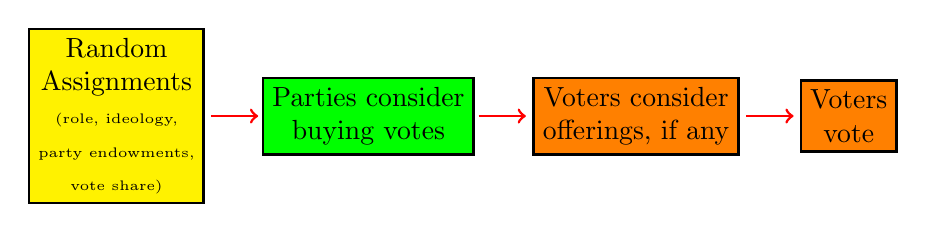
\begin{tikzpicture}[
                %scale=2
                scale=.2,
                line width=1pt] %

% random


                    % 1
                    \node[draw,align=center,fill=yellow,text=black] (RA) at (-22,-5.5) {Random\\Assignments\\\tiny{(role, ideology,}\\\tiny{party endowments,}\\\tiny{vote share)}}; % 1
                    \path [red,  ->] (-16,-5.5) edge (-13,-5.5);


                    % 2
                    \node[draw,align=center,fill=green,text=black] (OFFERP) at (-6,-5.5) {Parties consider\\buying votes}; % 1
                    \path [red,  ->] (1,-5.5) edge (4,-5.5);

                    % 3
                    \node[draw,align=center,fill=orange,text=black] (OFFERV) at (11,-5.5) {Voters consider\\offerings, if any}; % 1
                    \path [red,  ->] (18,-5.5) edge (21,-5.5);


                    % 3
                    \node[draw,align=center,fill=orange,text=black] (VDECID) at (24.5,-5.5) {Voters\\vote};


%%%%%%%%%%%%%%%%%%%%%%%%%%%%%%%%%%%%%%%%%%%%%%%%%%%%%%%%%%%%%%%%%%%%%%%%%%%%%%%%%%%%


\end{tikzpicture}

\end{document}